% 导言区
\documentclass{ctexart}

% 使用图片有以下几个部分要添加

% 导言区
%\usepackage{graphicx}

% 语法
% \includegraphics[<options>]{<file name>}

% 格式
% EPS, PDF, PNG, JPEG, BMP

\usepackage{graphicx}
\graphicspath{{fig/},{pics/}} % 图片在当前目录下的fig目录
% 这里面放的是图片的所在文件夹名字,可以存在多个文件夹,这边以fig和pics举例

% 正文区(文稿区)
\begin{document}
    \LaTeX{}中的插图:

    % 这里可以选择加后缀名也可以选择不用
    
\includegraphics[scale=0.3]{gura}
    
    % 这里的可选参数,比如说大小等,在前面的方括号内填写
    % 还有一些其他的可选参数调法,固定图像高度或者宽度
    
\includegraphics[height=2cm]{baiyu.jpg}

    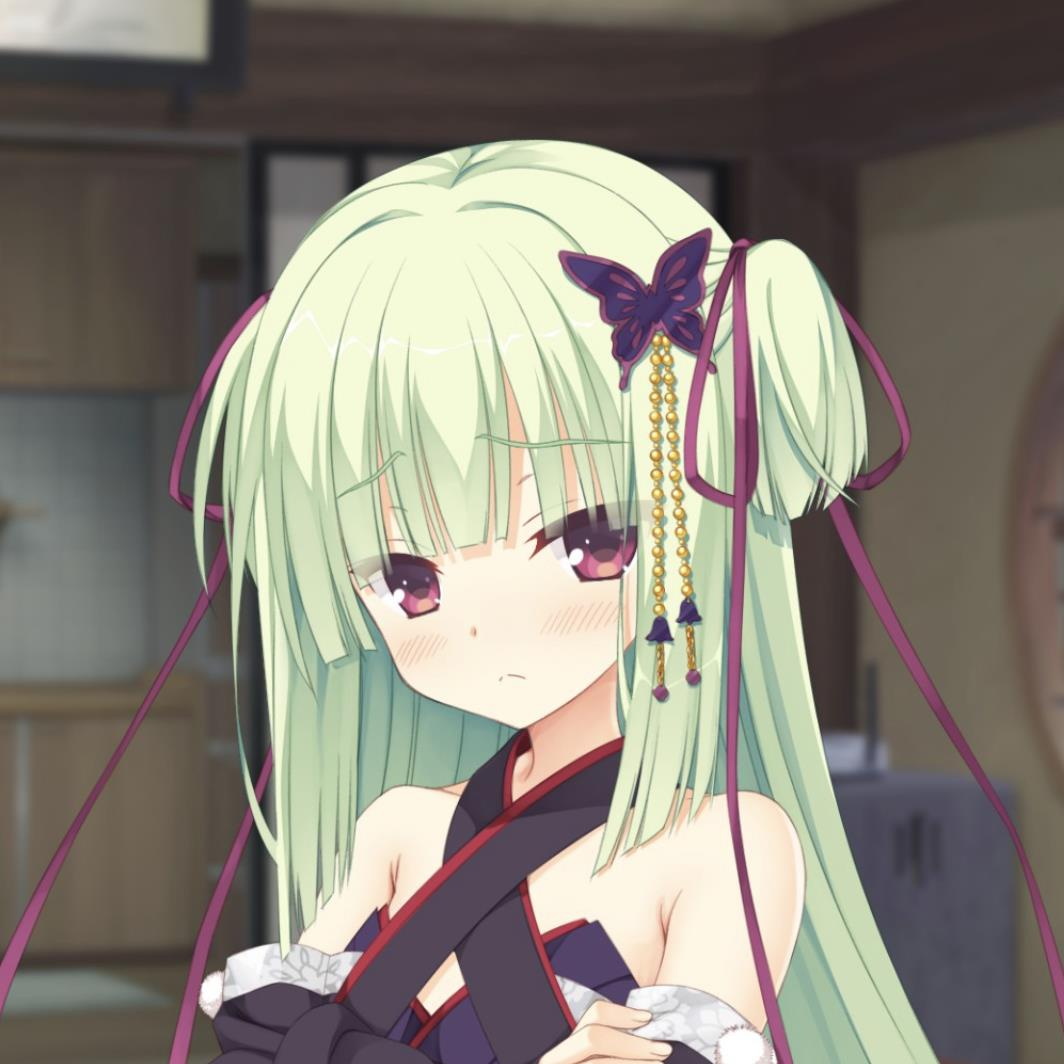
\includegraphics[width=8cm]{congyu.jpg}

    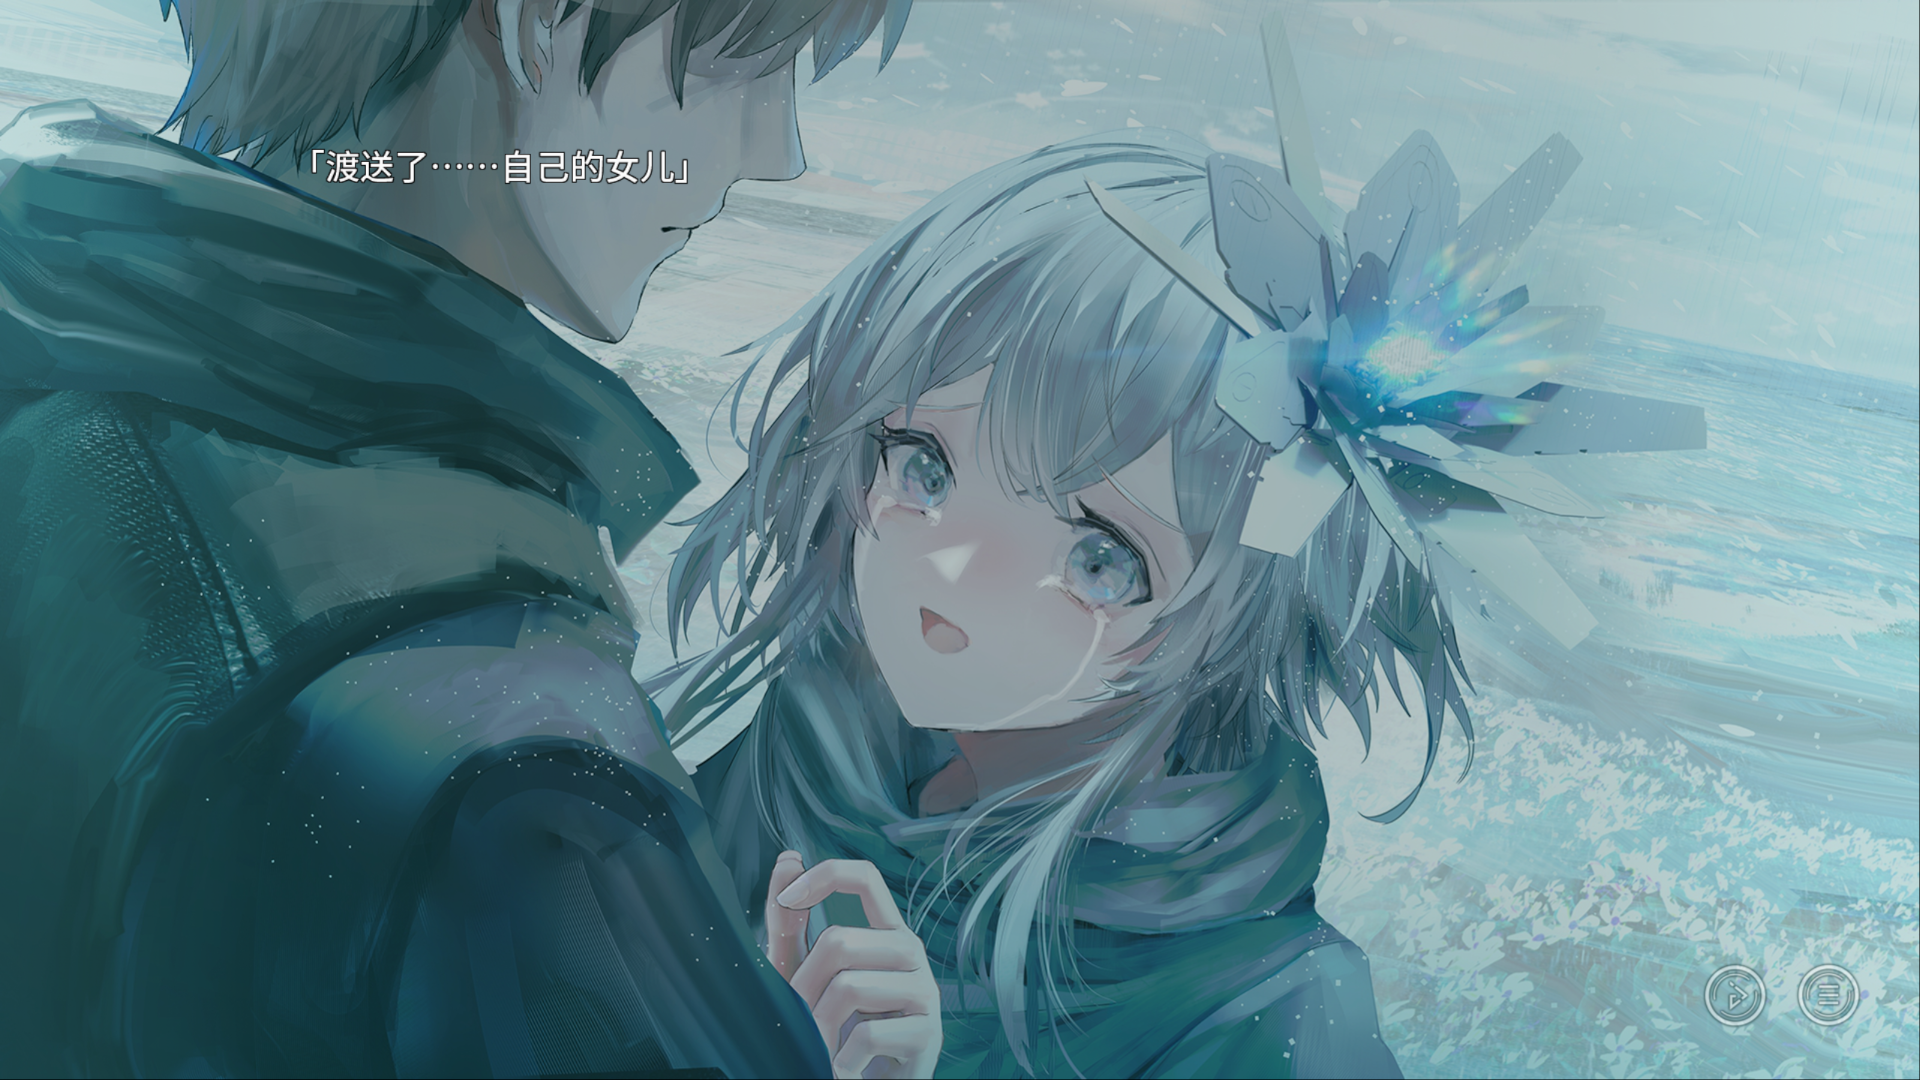
\includegraphics[width=1\textwidth]{1} % 以固定参照物来限制大小

    % 也可以设定更多的参数

    
\includegraphics[angle=45,width=0.2\textwidth]{2}

\end{document}

